\documentclass[a4paper,12pt,oneside,final]{extarticle}

\usepackage[utf8]{inputenc}
\usepackage[T1]{fontenc}

\usepackage{graphicx}
\usepackage{times}
\usepackage[english,swedish]{babel}

\usepackage{geometry}
\geometry{
 margin=20mm
} 

\usepackage{mathtools}
\usepackage{subcaption}
\usepackage{fancyhdr}
\usepackage{float}
\usepackage{titling}
\pagestyle{fancy}


\author{Fredrik Lindner, Sebastian Piwell, Aron Tornberg, Nicklas Fransson}
\title{Fluidsimulering i 2D, TNM085}



\begin{document}

\maketitle

\abstract{
 Den här rapporten avhandlar metoden SPH för fluider, samt implementering i C++.
 SPH är en överskådlig metod för att simulera traditionellt komplexa problem och är även enkel att implementera på modern hårdvara. 
}

\clearpage
\tableofcontents
\clearpage

\section{Bakgrund}
Historiskt sett så har det alltid varit intressant att studera hur fluider rör på sig.
När datorer började användas inom många industrier så kom möjligheten att sätta teorierna kring fluidsimulering i praktik.
Idag används det inom stora industriprocesser och för rena visuella tillämpningar.
Trots att datorer har gjort det möjligt att praktiskt simulera fluider så kvarstår det idag stora begränsningar på applicerbarheten.
Därför krävs det många förenkligar för att simuleringarna skall vara ett praktiskt verktyg.

\section{Syfte}
Projektets syfte är att skapa en 2-dimensionell vätskefluidsimulering i realtid för visualisering.
Vätskan skall gå att interagera med.
Eventuella förenklingar av fysiken kommer att göras för att uppnå snabbhet och stabilitet.

\clearpage

\section{Modell}
Rörelse i en fluid kan förklaras med Navier-Stokes ekvationer.
En fluid kan vara gas, vätska eller plasma.
Dessa ekvationer är baserade på Newtons andra lag och bevarar momentum, massa och är inkompressibel.
Ekvationen ger ett flödes fält som bestämmer hastigheten för en given punkt i tid och rum i fluiden.



%\section{Navier-Stockes}
%Navier-Stokes ekvationer
\begin{equation} \label{eq:navier-stokes-1}
\rho(\frac{\partial \vec{u}}{\partial t} + \vec{u} \cdot \nabla \vec{u}) =  -\nabla {\it p} + \nu \Delta \vec{u}
\end{equation}

\begin{equation}
\nabla \cdot \vec{u} = 0
\end{equation}

\begin{equation*}
\begin{aligned}
\begin{multlined}
\vec{u} = \mbox{hastighet} \\
\rho = \mbox{mass-densitet} \\
\it{p} = \mbox{tryck} \\
\nu = \mbox{viskositet} \\
\end{multlined}
\end{aligned}
\end{equation*}
Vänsterledet är produkten av mass-densiteter och accelerations-densiteter.
Högerledet är summan av kraft densiteterna.
I högerledet kan ekvationen utvecklas med externa krafter som gravitation och ytspänning.
Ekvationen under förklarar bevarandet av massan för en inkompressibel fluid.

I nästan alla fall är dessa ekvationer icke-linjära.
Det finns ännu inte något bevis att det alltid finns lösningar till dessa ekvationer i tre dimensioner.
Navier-Stokes ekvationer har varit och är fortfarande ett komplext matematiskt problem.

\section{Simulering}
Det finns två primära sätt att praktiskt simulera en fluid, Euleriskt och Lagraginskt(lol).
Den euleriska metoden går ut på att man har en fixed volym där man på bestämda positioner (celler) räknar ut fluidens egenskaper så som densitet, hastighet, tryck osv.
I den lagrangiska metoden behandlar man istället fluiden som en uppsättning partiklar som skulle kunna representera en molekyl av fluiden.
Varje partikel har egenskaper som hastighet, acceleration, position men även tryck och densitet.
Det Lagrangiska sättet att simulera fluider är vanligt och relativt enkelt att implementera.

“Smoothed Particle Hydrodynamics” (SPH)\cite{sph} är en Lagrangisk metod för att simulera fluider.
Den togs fram på 70-talet i syfte att lösa astrofysiska problem.
SPH delar upp fluiden i diskreta element (partiklar) där en bestämd “utjämningslängd” (även kallat interaktionsradie) jämnar ut partikelns egenskaper med hjälp av olka filterkärnor.
Vilken filterkärna som används beror på vilken egenskap som ska jämnas ut.
När en fluid representeras av en uppsättning partiklar så är mass-konserveringen given då det alltid finns en bestämd mängd partiklar med en bestämd massa.
Varje egenskap hos partikeln beräknas med avseende på alla andras egenskaper inom partikelns interaktionsradie.
\begin{figure}[H]
  \centering
    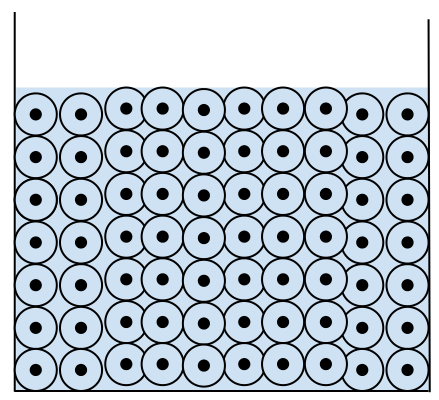
\includegraphics[width=0.5\textwidth]{bilder/partiklar_vila}
  \caption{En vätska representerad av partiklar med interaktionsradie.}
\end{figure}

\subsection{Mass-Densitet}
Massan för en partikel bestäms innan simuleringen och ses som en konstant.
För att bestämma mass-densiteten summeras massan för alla partiklar inom interaktionsradien och viktas med en filterkärna baserad på Gaussian (\ref{eq:w_def}).
Resultatet blir mass-densiteten kring partikeln.
\begin{equation}
\rho^{}_{i} = \sum_{\lim_{j}} {\it m_j W_{def} (r_i-r_j,h)}
\end{equation}

\begin{equation} \label{eq:w_def}
{\it W_{def} = \frac{315}{64 \pi h^9}(h^2-r^2)^3}
\end{equation}

\subsection{Krafter}
\subsubsection{Tryck}
Trycket är den första delen av högerledet i Navier Stokes ekvation.
Trycket kan bestämmas med den idella gas lagen:
\begin{equation}
{\it pV = nRT}
\end{equation}
där V är volymen per en enhets massa, n är antalet partiklar i mol, R är den universiella gas konstanten och T är temperaturen.
Högerledet är konstant för simuleringar denna rapport avser och kan därför sättas till en styvhets konstant k. 
För att få attraherande krafter måste ta hänsyn till vilodensiteten. Uttrycket för trycket blir då:

\begin{equation}
{\it p = k(\rho - \rho^{}_{0})}
\end{equation}


För att få en inkopresibel fluid behöver styvhetskonstanten k vara så hög som möjligt. Det betyder att ingen partikel ska kunna gå in i den andra. Detta kan bli ett problem vilket tas upp senare i rapporten.

För att bestämma kraften från trycket summeras trycket hos partiklar inom interaktionsradien på liknande sätt som för mass-densiteten (\ref{eq:f_tryck}).
Viktningskärnan som används för denna summering är tillskillnad från mass-densiteten nu mycket snävare och spetsig (\ref{eq:w_tryck}).
För att få en jämnare kraftfördelning som mer följer Newtons 3de lag används följande summering.

\begin{equation} \label{eq:f_tryck}
f^{tryck}_i = - \sum_{j \neq i} \frac{\it p_i + p_j}{2} \frac{m_j}{\rho^{}_{i} \rho^{}_{j}} \nabla {\it W_{tryck} (r_i - r_j,h)}
\end{equation}

\begin{equation} \label{eq:w_tryck}
{\it W_{tryck} = -\frac{45}{\pi h^6}\frac{(h-r)^2}{r}} \vec{r}
\end{equation}


\begin{figure}[H]
  \centering
    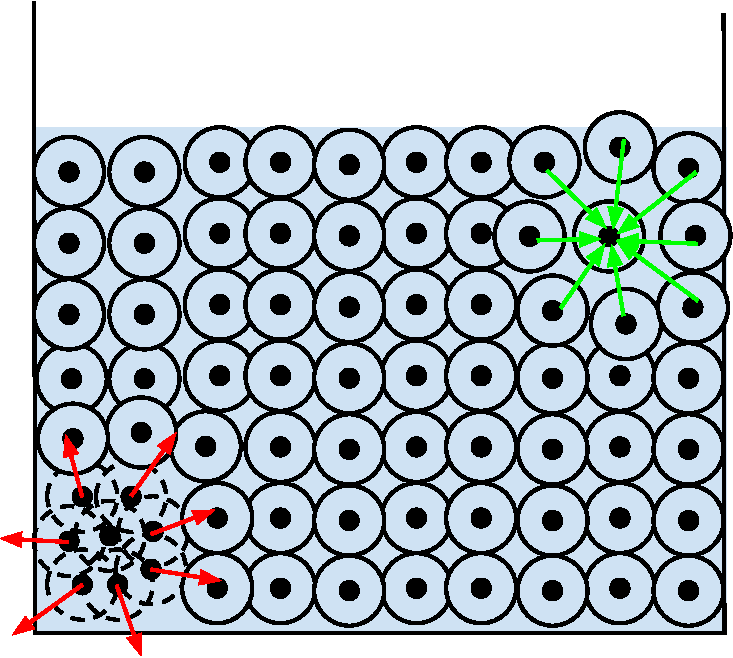
\includegraphics[width=0.5\textwidth]{bilder/partiklar_komprimering}
  \caption{Partiklar som verkar på andra partiklar.}
\end{figure}



\subsubsection{Viskositet}
Viskositeten är den andra delen av högerledet i Navier-Stokes ekvation (\ref{eq:navier-stokes-1}).
Viskositeten står för strömningsmotståndet i fluiden.
Den uppkommer ifrån friktionen mellan partiklarna och minskar den relativa hastigheten mellan dem.
Viskositetens storlek bestämms av en konstant som beror på vilken typ av fluid man ska simulera.
Kraften som viskositeten påverkar partikeln med fås av uttrycket:
\begin{equation}
f^{viskositet}_i = \mu \sum_{j} {\it \frac{m_j}{\rho^{}_{i} \rho^{}_{j}} (u_j - u_i) \nabla^{2}_{} W_{viskositet} (r_i - r_j,h)}
\end{equation}

\begin{equation}
{\it W_{viskoitet} = \frac{45}{\pi h^6} {(h-r)}}
\end{equation}

Där den relativa hastigheten används för att få en symetrisk kraft som föjer Newtons 3de lag. Viktningsknärnan är alltid positiv för att alltid fungera som en dämpningsterm och inte tillsätta energi i systemet och göra det ostabilt. 

\subsubsection{Gravitation}
Gravitationen påverkar alla partiklar lika mycket enligt uttrycket:
\begin{equation}
f^{gravitation}_{i} = \rho^{}_{i}g
\end{equation}
Där g är gravitationsaccelerationen som verkar i negativt y-led i simuleringen.

\subsection{Kollisionshantering}
\subsubsection{Väggar}
För att inte partiklarna ska försvinna utanför simuleringsrymden har enkla väggar vid kanterna skapats.
Vid väggarna sker en kollisionshantering som aktiveras då partiklarna är tillräckligt nära.
Kollisionsresponsen beror på styvheten på vätskan och infallsvinkeln.
Den uppdaterar partikelns acceleration vilket simulerar en vägg.
\begin{figure}[H]
  \centering
    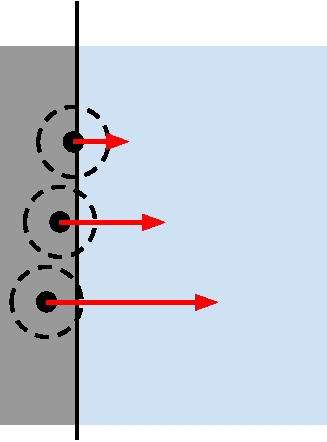
\includegraphics[width=0.3\textwidth]{bilder/partiklar_vagg}
  \caption{Partiklar som får en acceleration från vägg.}
\end{figure}

\subsubsection{Kollisionspartiklar}
I simuleringen kan man lägga till kanter i form av kantpartiklar.
Kantpartiklarna defineras som de andra partiklarna men med tyngre massa, därmed större mass-densitet och tryck.
De funkar som de andra partiklar förutom att deras position inte ändras.
Med deras tunga massa och fix positionering fungerar de som kanter.
I en offline simulering räcker denna definering av kanter.
Men för en interaktiv simulering kan inte tidssteget vara tillräckligt litet för att det ska fungera bra.
För enstaka partiklar eller partiklar med höga hastigheter hinner inte kantpartiklarna påverka de inkommande partiklarna.
Partiklarnas hastighet förändras då inte och åker igenom kanten. 

\begin{figure}[H]
  \centering
    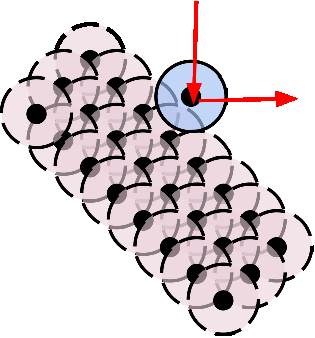
\includegraphics[width=0.3\textwidth]{bilder/partiklar_kolpart}
  \caption{Kantpartiklar}
\end{figure}

För att få bättre kanter i en realtids simulering behövs en omedelbar verkan på partikelns hastighet då de träffar kanten.
Det fås genom att updatera partiklarnas hastighet på ett annat sätt då de är inom kantpartiklarnas interaktionsområde.
Istället för Navier Stokes ekvation för updatering av hastigheten används en enkel partikel mot partikel kollesionshantering.
En reflektionsvinkel beräknas mellan partiklarna och hastigheten updateras i den riktningen.

\subsection{Integrering}
För updateringa av position och hastighet har integreringsmetoden Leap-Frog används. Den fungerar genom att ta halva steg för positionen och hastigheten.
Hastigheten börjar ett halvt steg bakåt.
I och med det så “hoppar” positionen och hastigheten över varandra.
Hastigheten för den aktuella tiden fås approximativt av halvstegen bakom och framför.
Det är en stabil och snabb integreringsmetod som lämpar sig till simuleringen.

\begin{equation}
{\it u_{t + \frac{1}{2} \Delta t} = u_{t - \frac{1}{2} \Delta t} + \Delta t a_t}
\end{equation}
\begin{equation}
{\it r_{t+ \Delta t} = r_t + \Delta t u_{t + \frac{1}{2} \Delta t }}
\end{equation}

\begin{equation}
{\it u_{-\frac{1}{2} \Delta t} = u_{0} + \frac{1}{2} \Delta t a_0}
\end{equation}

\begin{equation}
{\it u_t \approx \frac{u_{t - \frac{1}{2} \Delta t} + u_{t + \frac{1}{2} \Delta t} }{2} }
\end{equation}

\clearpage
\section{Implementering}
Två steg används för att lösa detta problem.

I steg ett delas simuleringen upp i ett rutnät med höjd och bredd lika med interaktionsradien med en lista kopplad till varje cell i rutnätet.
Varje partikel i systemet koppas till den lista vars cell partikeln befinner sig i.

I steg två kontrolleras vilka andra partiklar som befinner sig inom interaktionsradien till varje partikel och dessa placeras i en lista av grannar till partikeln i fråga.
För att undvika kvadratisk tidskomplexitet i denna kontroll använder man det faktum att samtliga partiklar som är grannar till en specifika partikel antingen kommer befinna sig i samma cell som partilen i fråga eller någon av de 8 omkringliggande cellerna och utför enbart kontrollen för listorna kopplade till dessa 9 celler samt så begränsas antalet grannar i listan till 64.

I uträkningen av hydrodynamiken används sedan endast de partiklar som finns i listan av grannar för den aktuella partikeln.
Vilket minskar tidskomplexiteten markant.

Vid beräkningen av hydrodynamiken så beror varje partikels tillstånd enbart på tillståndet för partiklarna i föregående tidssteg.
Det finns alltså inga teoretiska hinder för räkna ut hydrodynamiken för samtliga partiklar samtidigt.

OpenMP \cite{openmp} har används för att räkna på flera partiklar samtidigt.
\textit{pragma}-direktiv har placerats innan de lopar som itererar genom partiklarna för att istruera kompilatorn om att dessa lopar kan köras parallellt på centralprocessorn.

\section{Rendering}
För att rita simuleringen skickas en lista med koordinater för samtliga partiklar via OpenGL till grafikkortet.
Två olika ritlägen finns i simuleringen.
Dels ett punktläge där varje partikel helt enkelt ritas ut som en punkt och dels metaball-läget.

I metaball läget används metaballs för att rita ut partiklarna.
Metaballs fungerar på så sätt att man för varje partikel definierar en radialt avtagande funktion.
Förje punkt i simuleringsmiljön summerar man sedan dessa funktioner och kollar ifall summan är över ett tröskelvärde.
Om den är över tröskelvärdet säger man att punkten är fylld och annars tom.
På detta sätt kan man representera partiklar som bollar som har egenskapen att de ser ut att smälta ihop då de kommer nära varandra.
Så kallade \textit{metaballs}.

Implementationen av metaballs i denna simuleringen fungerar på så sätt att varje partikel ritas ut som en pointsprite vars textur definieras av en fragment-shader (gradientball.frag) som texturerar pointspriten som en radialtavtagande gradient enligt funktionen:
\begin{equation}
r^{4} -r^{2} + 0.25
\end{equation}
Som en optimeringsåtgärd räknas $ r^{2} $ ut genom att ta skälarprodukten av den vektor som går mellan bildpunkten och partikelnskoordinater med sig själv.

Istället för att rita partiklarna till skärmen så används efterbehandling.
Bilden renderas istället till en textur som behandlas i en fragment-shader (metaballs.frag) för att sedan ritas på skärmen.
I fragment-shadern så sätts alpha-värdet på texturen dels så att värden under tröskelvärdet sätts till noll men också på så att en mjuk övergång sker för att undvika en skarp pixlig kant.
En normalkarta beräknas även genom att tolka den ingående texturen som en höjdkarta.
Normalkartan används för att räkna ut diffust ljus till som används för att bestämma texturens RGB-värden.
På så sätt åstadkoms en 3D-effekt på vätskan.
\clearpage

\section{Resultat}
Den interaktiva applikationen som togs fram för att demonstrera simuleringen klarar av att simulera och visa ca 16000st partiklar samtidigt.
Det gjordes ett flertal olika begynnelsevillkor för fluiden.
I några fall släpptes vätskan ifrån en höjd för att studera hur komprimerad vätskan blev.
Det testades också att distribuera ut vätskan över tid, ungefär som en vattenspridare.

\begin{figure}[H]
\centering
  \begin{subfigure}[b]{.4\textwidth}
      \setlength\fboxsep{0pt}
      \setlength\fboxrule{0.5pt}
      \fbox{
\includegraphics[width=\textwidth]{bilder/dam_break}}
  \end{subfigure}
  ~
  \begin{subfigure}[b]{.4\textwidth}
      \setlength\fboxsep{0pt}
      \setlength\fboxrule{0.5pt}
      \fbox{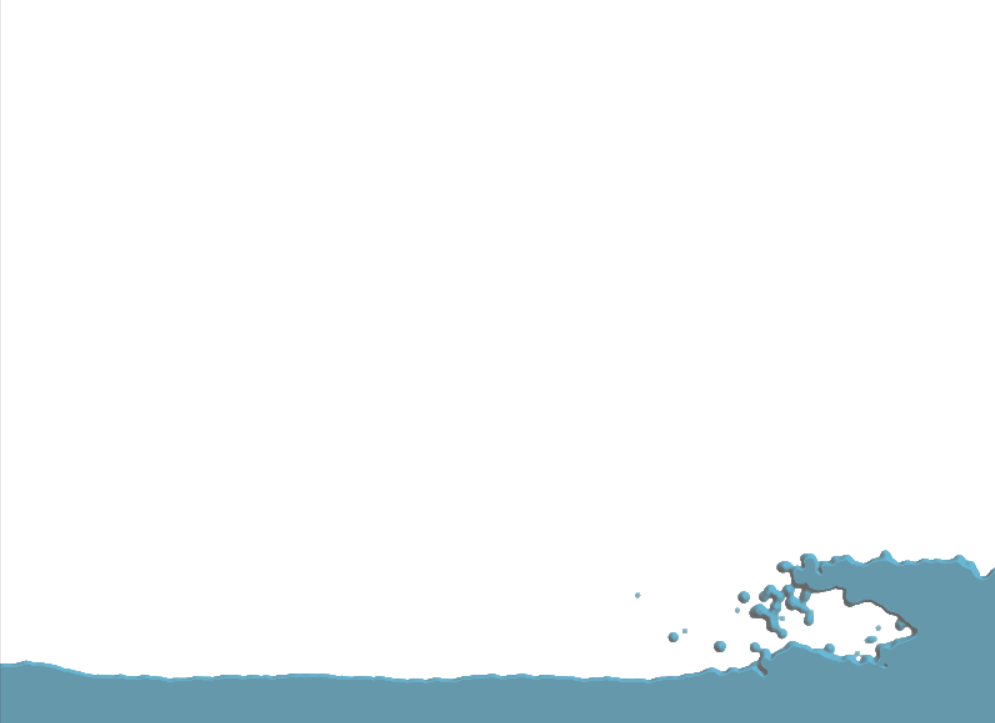
\includegraphics[width=\textwidth]{bilder/koolWave}}
  \end{subfigure}
\caption{Ett vanligt testfall, \textit{dam break}, vid olika tidpunkter.}
\end{figure}

\begin{figure}[H]
  \centering
    \setlength\fboxsep{0pt}
    \setlength\fboxrule{0.5pt}
    \fbox{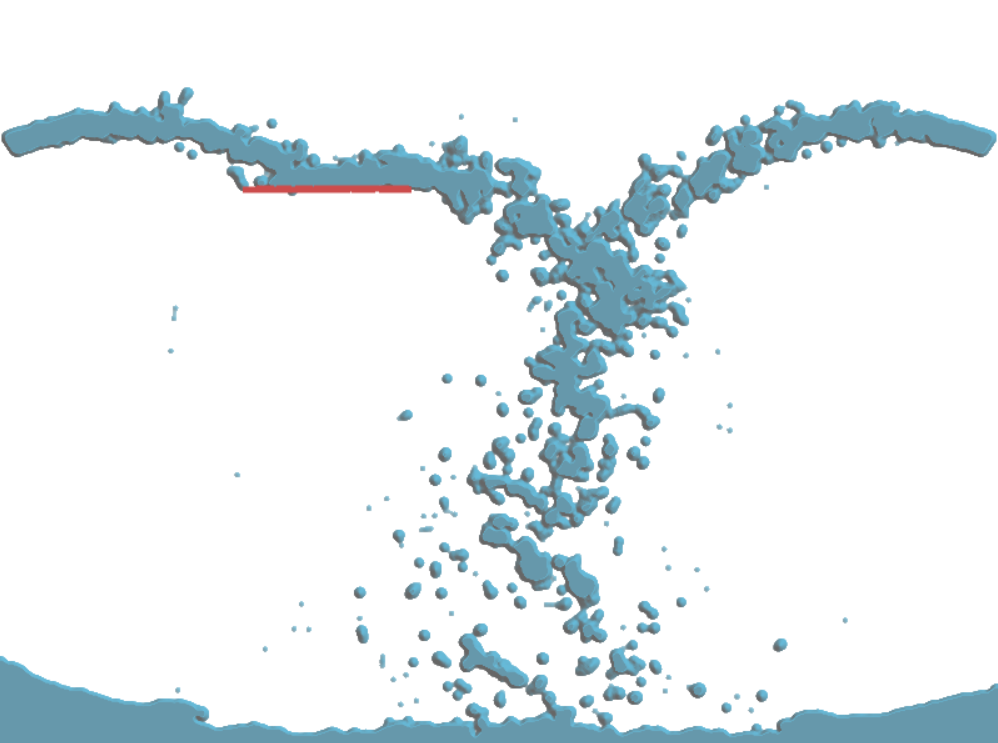
\includegraphics[width=0.8\textwidth]{bilder/emiters}}
  \caption{Exempel på partikelkälla och kantpartiklar.}
\end{figure}

\clearpage

\section{Diskussion}
\subsection{Begränsningar}
SPH medför begränsningar både på snabbhet och styvhet hos en fluid.
För att simulera t.ex vatten som är en inkompressibel vätska så krävs det mycket hög styvhet.
En hög styvhet medför att dynamiken på systemet måste vara väldigt snabbt, vilket i sin tur medför att steglängden i simuleringen måste vara väldigt kort.

Att få ett interaktivt system som använder metoden SPH för att simulera en fluid är ofta en avvägning mellan styvhet och hastighet på systemet. 
\subsection{Förbättringar}
Ett flertal förbättringar när det kommer till stabilitet/styvhet och hastighet kan göras.
\subsubsection{GPGPU}
GPGPU (General-purpose computing on graphics processing units) kan tillämpas för att ytterligare parallellisera beräkningarna.
Modern grafikhårdvara är speciellt gjord för att göra enkla beräkningar parallellt och därmed skulle man kunna beräkna på fler partiklar parallellt.

\subsubsection{PCISPH}
PCISPH (predictive-corrective incompressible SPH)[REFERENS] är en utökad SPH-metod.
Metoden försöker att approximera hur trycket skall ändras utan att faktiskt beräkna trycket.
Detta gör att ett större tidssteg kan användas utan att systemet stabilitet påverkas.

Det finns även andra metoder baserade på SPH som lyckas bibehålla en hög styvhet utan att påverka stabiliteten på systemet, tex Constraint Fluids\cite{bodin} av Bodin et. al.

% \section{Krafter}
% \subsection{Mass-Densitet}

% \begin{equation}
% \rho^{}_{i} = \sum_{\lim_{j}} {\it m_j W_{def} (r_i-r_j,h)}
% \end{equation}

% \begin{equation}
% {\it W_{def} = \frac{315}{64 \pi h^9}(h^2-r^2)^3}
% \end{equation}

% \subsection{Tryck}
% Ideal gas law
% \begin{equation}
% {\it pV = nRT}
% \end{equation}
% Tryck tärm
% \begin{equation}
% {\it p = k(\rho - \rho^{}_{0})}
% \end{equation}
% Tryck kraft
% \begin{equation}
% f^{tryck}_i = - \sum_{\lim^{}_{j \neq i}} \frac{\it p_i + p_j}{2} \frac{m_j}{\rho^{}_{i} \rho^{}_{j}} \nabla {\it W_{tryck} (r_i - r_j,h)}
% \end{equation}

% \begin{equation}
% {\it W_{tryck} = -\frac{45}{\pi h^6}\frac{(h-r)^2}{r}} \vec{r}
% \end{equation}

% \subsection{Viskositet}
% \begin{equation}
% f^{viskositet}_i = \mu \sum \limit^{}_{j} {\it \frac{m_j}{\rho^{}_{i} \rho^{}_{j}} (u_j - u_i) \nabla^{2}_{} W_{viskositet} (r_i - r_j,h)}
% \end{equation}

% \begin{equation}
% {\it W_{viskoitet} = \frac{45}{\pi h^6} {(h-r)}}
% \end{equation}

% \subsection{Gravitation}
% \begin{equation}
% f^{gravitation}_{i} = \rho^{}_{i}g
% \end{equation}

% \section{Leap-frog}
% \begin{equation}
% {\it u_{t + \frac{1}{2} \Delta t} = u_{t - \frac{1}{2} \Delta t} + \Delta t a_t}
% \end{equation}
% \begin{equation}
% {\it r_{t+ \Delta t} = r_t + \Delta t u_{t + \frac{1}{2} \Delta t }}
% \end{equation}

% Initial velocity
% \begin{equation}
% {\it u_{- \frac{1}{2} \Delta t} = u_{0} + \frac{1}{2} \Delta t a_0}
% \end{equation}

% Approx
% \begin{equation}
% {\it u_t \approx \frac{u_{t - \frac{1}{2} \Delta t} + u_{t + \frac{1}{2} \Delta t} }{2} }
% \end{equation}

\clearpage

\begin{thebibliography}{9}
  
\bibitem{sph}
  R.A. Gingold and J.J. Monaghan, \emph{Smoothed particle hydrodynamics: theory and application to non-spherical stars}, Mon. Not. R. Astron. Soc., Vol 181 1977
\bibitem{kelager}
  Micky Kelager, \emph{Lagrangian Fluid Dynamics Using Smoothed Particle Hydrodynamics}, University of Copenhagen, 2006
\bibitem{openmp}
  http://openmp.org/
\bibitem{bodin}
   K. Bodin, C. Lacoursière, M. Servin, \emph{Constraint Fluids}, IEEE Transactions on Visualization and Computer Graphics, Jan 2011 
\end{thebibliography}


\end{document}